\chapter{Adaptación GPU}


\section{Convolución como GEMM \label{Intro_GEMMM}}

\begin{figure}[H]
	\centering
	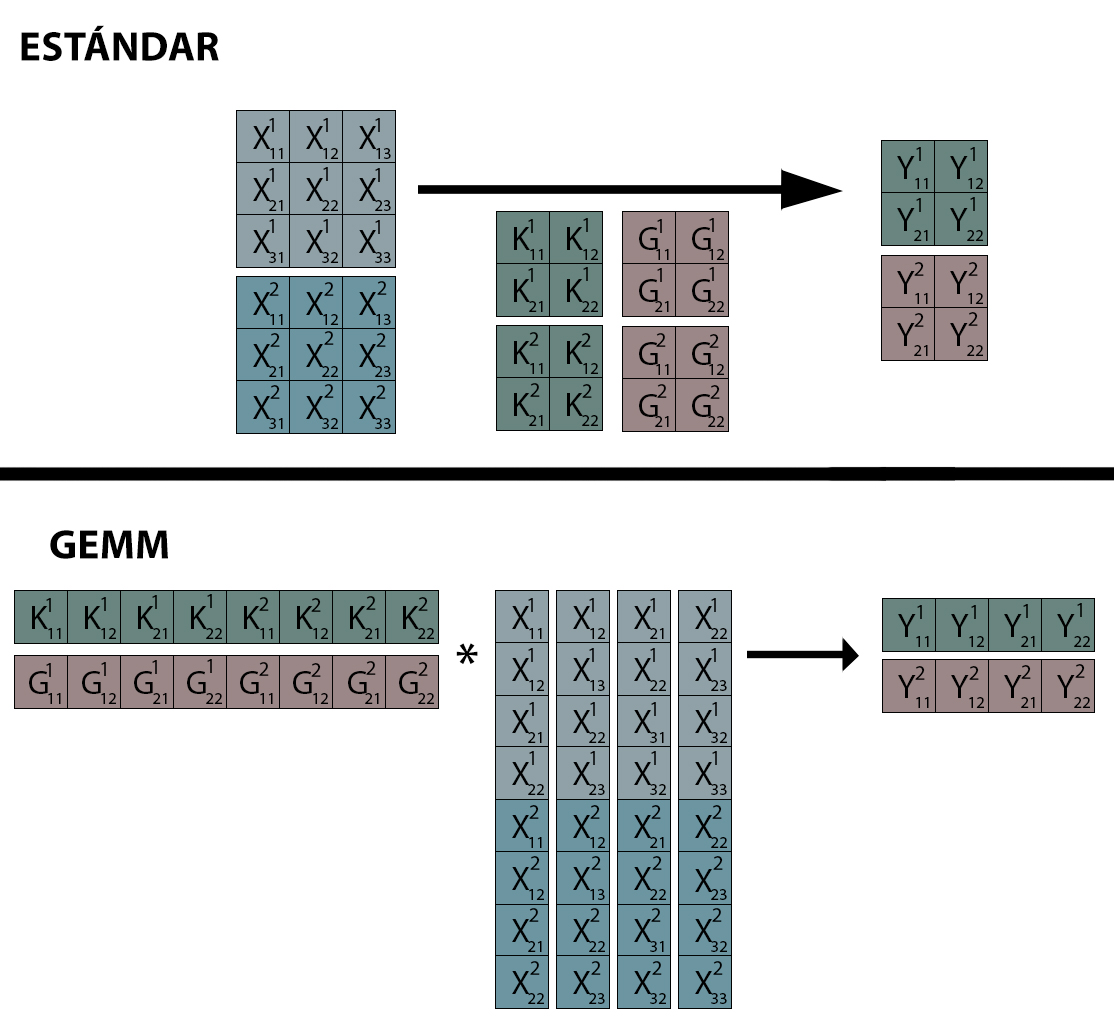
\includegraphics[scale=0.35]{imagenes/conv_std_vs_gemm.jpg}  
	\caption{Imagen de una convolución estándar frente a una convolución empleando GEMM}
	\label{fig:conv_std_vs_gemm}
\end{figure}
Se trata de un enfoque ampliamente conocido en el mundo de deep learning, empleándolo gran cantidad de librerías del sector como Caffe, Torch-cunn, Theano-CorrMM, o incluso CuDNN. \cite{conv_GEMM_FFT_comparacion} \\
El enfoque GEMM (General Matrix Multiply o Multiplicación General de Matrices) en redes neuronales convolucionales permite reducir el tiempo de cómputo requerido en una convolución a cambio de aumentar el espacio necesario para la misma. Este método consiste en ``desenrrollar'' tanto el volumen de entrada X como la matriz de filtros K, además de realizar una serie de duplicaciones en X, de tal forma que cada columna de esta nueva matriz 2D X\_unroll contenga todos los elementos de X implicados en el cálculo de una posición distinta del volumen de salida Y. Como los resultados de cada convolución se suman a lo largo de cada canal de profundidad, estos se pueden concatenar en una matriz de gran tamaño. De esta forma, cada kernel de pesos se transforma en una fila de una gran matriz de pesos, tal y como se muestra en la figura \ref{fig:conv_std_vs_gemm} con los kernels K y G (colores verde y marrón). \\
Mientras que el método estándar requiere de varias iteraciones para calcular cada valor del volumen de salida Y (figura \ref{fig:forward_prop_convolucional}), en la parte inferior de la figura \ref{fig:conv_std_vs_gemm} se observa como la alternativa GEMM permite que cada valor de Y sea el resultado de multiplicar una fila de pesos (K o G en la figura \ref{fig:conv_std_vs_gemm}) por una columna de X\_unroll (azul). \cite{Programming_Massively} \\
De esta forma, con N kernels de tamaño KxK, un volumen de entrada con C canales de profundidad, y un volumen de salida de dimensiones $NxH_{out}xW_{out}$, una multiplicación matricial entre la matriz de pesos $M_1$ con N filas y $K^2*C$ columnas, y X\_unroll con $K^2*C$ filas y $H_{out}*W_{out}$ columnas, produce el mismo volumen de salida Y que una convolución ordinaria con N kernels distintos. \\
Por último, aunque se haya omitido para simplificar la comprensión del método planteado, tras realizar dicha multiplicación matricial se debe sumar el sesgo y aplicar la función de activación correspondiente a cada elemento del volumen de salida Y.

\subsection{Memoria requerida al emplear GEMM}

Al realizar una convolución, un mismo filtro de pesos puede iterar más de una vez por varios valores de X. Esto implica la duplicación dichos valores de X en la matriz X\_unroll tantas veces como se requiera el acceso a los mismos. En el caso de una entrada X(3x3) y un kernel de pesos K(2x2) (ejemplo de la figura \ref{fig:conv_std_vs_gemm}), el valor central de X deberá duplicarse 4 veces, mientras que el valor central de cada lateral se duplicará 2 veces y los valores de cada esquina solo requieren 1 acceso por lo que no  se duplican. Así, una matriz inicial X(3x3) con 9 valores, se transforma en X\_unroll con 4*1 + 2*4 + 1*4 = 16 valores, contando con un ratio de expansión de 16/9 = 1.8 . \\
 Como cada valor de salida $Y^m_{ij}$ es producto de una convolución de K*K pesos a lo largo de X sobre C canales de profundidad, el número de columnas de X\_unroll se define por C*K*K. De la misma forma, como el resultado de cada fila multiplicada por cada columna de las matrices ``desenrolladas'' aportan un valor $Y^m_{ij}$, X\_unrolled tiene tantas columnas como Y elementos ($M*H_{out}*W_{out}$). \\
 El ratio de expansión se define mediante $\frac{C*K*K*H_{out}*W_{out}}{C*H*W}$, donde H y W hacen referencia a las filas y columnas de X, y $H_{out}$ y $W_{out}$ a las filas y columnas de la salida $Y$ respectivamente. En general, si la entrada X y la salida Y poseen unas dimensiones mucho más grandes que el filtro de pesos K, el ratio de expansión será de K*K. \\
 Dado que cada kernel de pesos presenta unas dimensiones de K*K y se representa como una fila en la matriz total de pesos, esta tendrá K*K filas y M columnas, siendo M el número de filtros de pesos a aplicar sobre X. \\
 Realizar varias convoluciones sobre una misma entrada X(una con cada filtro de pesos distinto) implica compartir una única matriz X\_unrolled. Sin embargo, para valores comunes de filtros de pesos (5 o superior), una matriz de entrada con dimensiones expandidas con un ratio de K*K puede ser excesivamente grande. Como el consumo de memoria por almacenar todas las matrices de entrada expandidas en un minibatch puede suponer un problema, simplemente se reservará un espacio de $C*K*K*H_{out}*W_{out}$ (una instancia de X\_unrolled), de forma que se reutilice para cada dato del minibatch. \cite{Programming_Massively}

\section{Retropropagación GEMM en capa convolucional}

En la figura \ref{fig:conv_backprop_como_convolucion_Y_K_pad} se vio como la retropropagación respecto a la entrada en una capa convolucional consistía en una convolución entre los kernels de pesos y el volumen de salida. Del mismo modo, en la figura \ref{fig:conv_backprop_como_convolucion_Xpad_Y} también se mostró como el gradiente respecto a los pesos consistía en una convolución entre el volumen de entrada y el de salida. \\
Como ambos gradientes se pueden implementar como convoluciones, y en la sección \ref{Intro_GEMMM} se mostró como implementar convoluciones con el enfoque GEMM, la retropropagación en una capa convolucional se puede implementar mediante el enfoque GEMM.

\begin{figure}[H]
	\hspace{-25mm}
	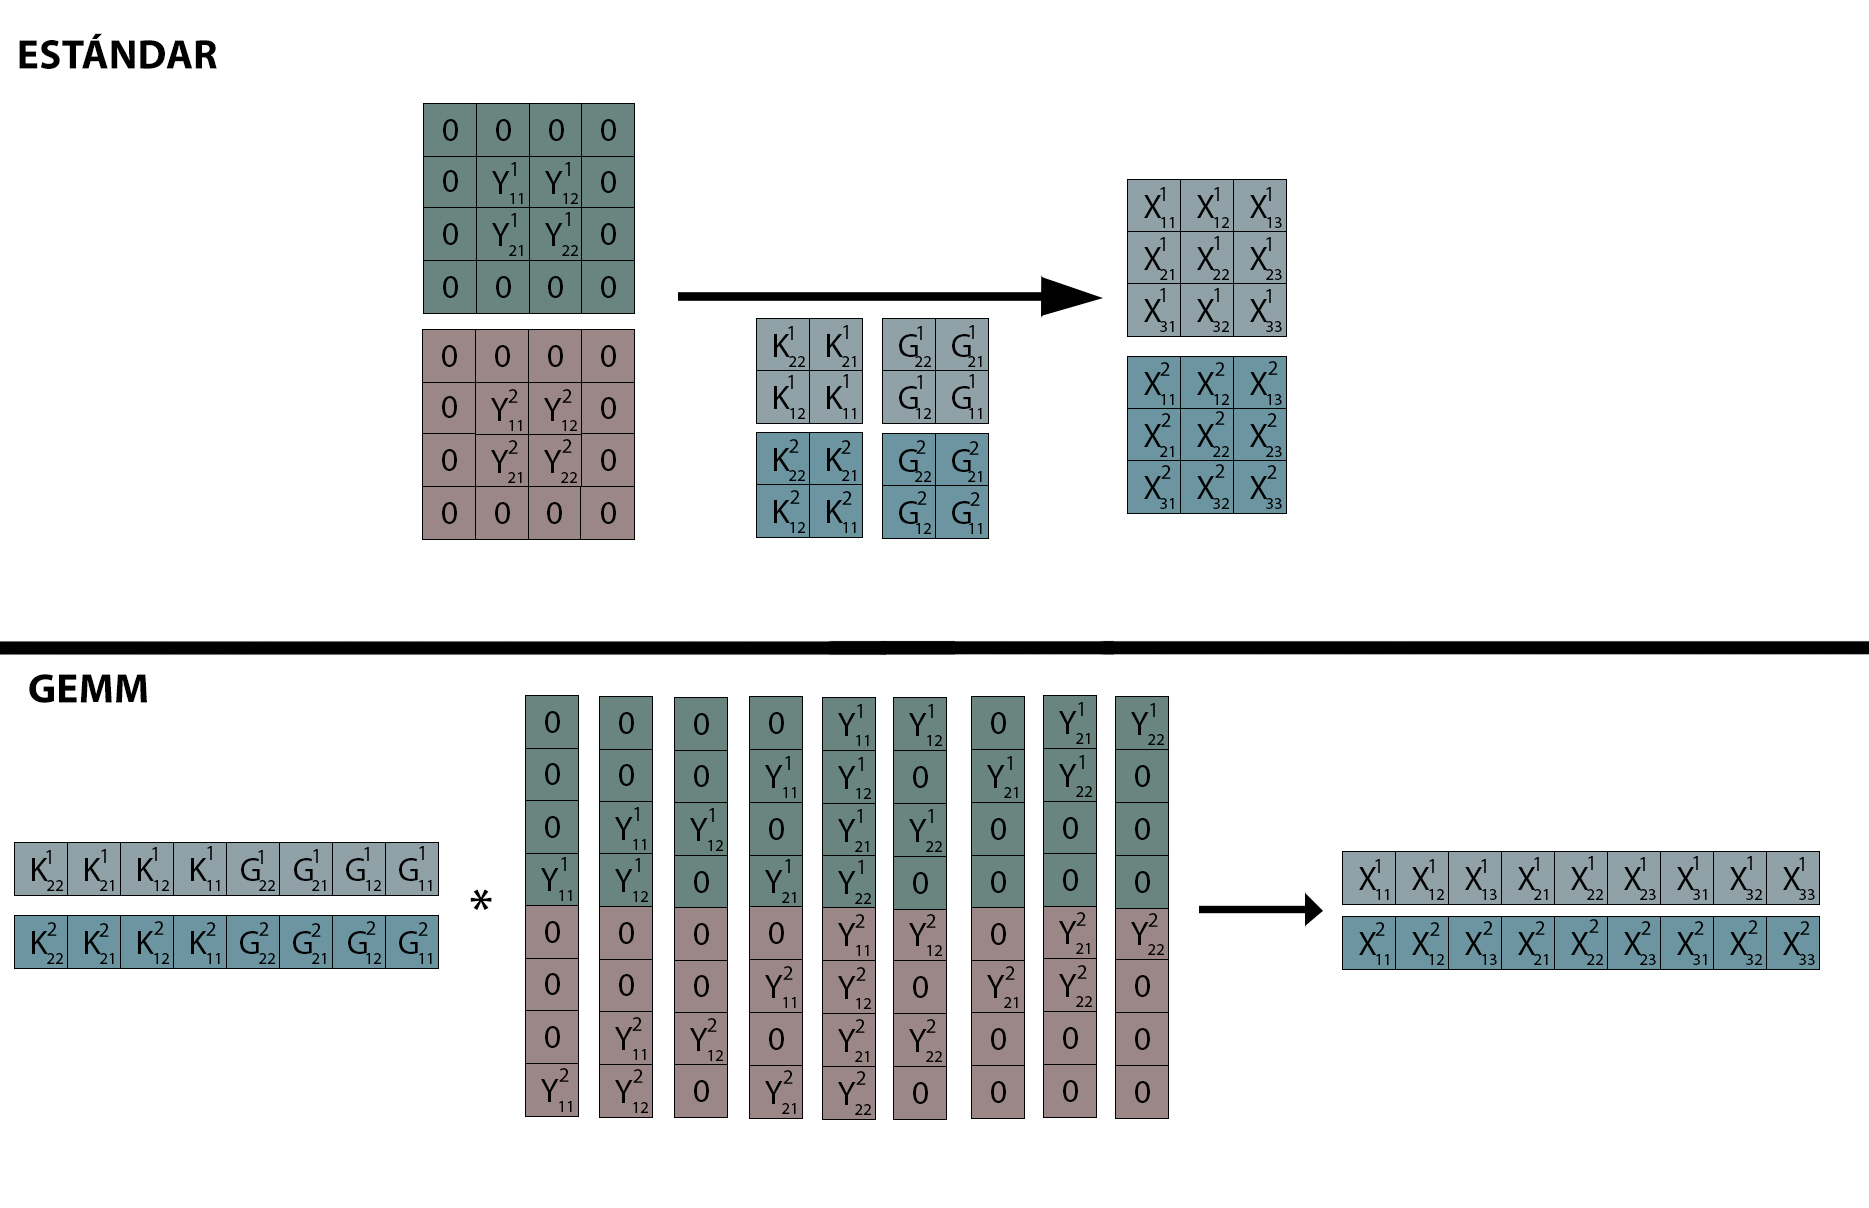
\includegraphics[scale=0.3]{imagenes/conv_std_vs_gemm_backprop.jpg}  
	\caption{Retropropagación en una capa convolucional de forma estándar frente a GEMM respecto a la entrada}
	\label{fig:conv_std_vs_gemm_backprop}
\end{figure}

\begin{figure}[H]
	\hspace{-25mm}
	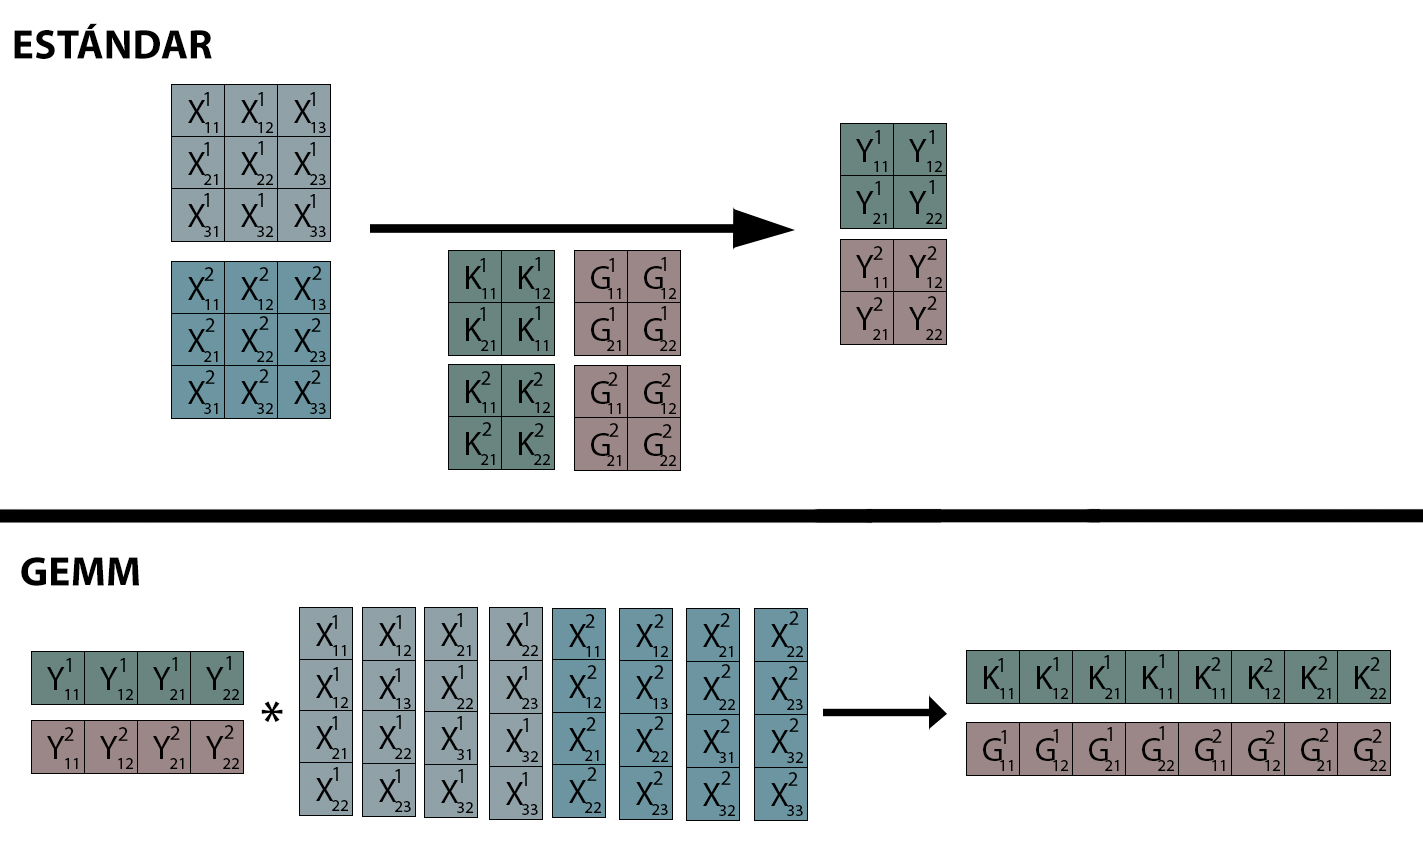
\includegraphics[scale=0.3]{imagenes/conv_std_vs_gemm_backprop_pesos.jpg}  
	\caption{Retropropagación en una capa convolucional de forma estándar frente a GEMM respecto a los pesos}
	\label{fig:conv_std_vs_gemm_backprop_pesos}
\end{figure}

\section{CUDA}
CUDA es una plataforma de cómputo paralelo de propósito general y modelo de programación que aprovecha la capacidad computacional de las GPUs de NVIDIA para resolver gran cantidad de problemas computacionalmente costosos de manera eficiente. CUDA permite acceder a la GPU de forma similar al común acceso a CPU que experimenta un desarrollador promedio. \\
El modelo de programación CUDA permite ejecutar aplicaciones en sistemas de computación heterogéneos, caracterizándose estos por CPUs y GPUs, cada uno con su propia memoria separada por un bus PCI-Express. \\
Cuando se lanza una función kernel desde CPU, la ejecución se traslada a GPU, esta genera un gran número de hebras y cada una de ellas ejecuta las órdenes especificadas en dicho kernel. \\
Las hebras se organizan en una cuadrícula o grid compuesta por varios bloques de hebras. De esta forma, cada hebra pertenece a un bloque de hebras, y cada bloque de un mismo kernel pertenece a un mismo grid. Todas las hebras de un mismo grid comparten la misma memoria global. Por tanto, hebras de distintos grids no pueden cooperar. A su vez, las hebras de un mismo bloque se pueden sincronizar y compartir memoria a nivel de bloque, siendo esta más escasa pero presentando una latencia considerablemente menor que la memoria global. CUDA organiza los grids y bloques mediante estructuras que pueden ser 1D, 2D o incluso 3D.
\subsection{Multiplicación de matrices en CUDA}

Dadas dos matrices A(MxK) y B(KxN), se obtiene C(KxN) como producto de la multiplicación AB. Basándome en mi propia experiencia, una primera aproximación de cara a realizar dicha operación en CUDA consiste en crear un bloque Block(KxN), de forma que cada hebra calcule una posición de la matriz resultado C. Dada la naturaleza extremadamente simple de tal implementación, el desarrollador que la llevó a cabo optará por buscar formas de reducir el tiempo de cómputo requerido por la misma, optando en la mayoría de los casos por emplear memoria compartida de bloque. Tras desarrollar esta ``segunda versión'', el siguiente paso del desarrollador consiste en comparar ambas implementaciones para verificar si efectivamente se obtiene una ganancia notable sobre la primera. En el proceso se observa como para matrices de tamaño reducido ambas implementaciones parecen funcionar. Sin embargo, a medida que aumenta el tamaño de las mismas se ve un claro ``tope'' pues ambas comparten un mismo defecto, el tamaño de bloque. Por ejemplo, para calcular C(50x50) = A(50x10) x B(10x50) ambas implementaciones requerirían un bloque de 50x50 = 2500 hebras, lo cual es imposible pues excede el tamaño límite (CUDA solo permite 1024 hebras por bloque). \\

\begin{figure}[H]
	\centering
	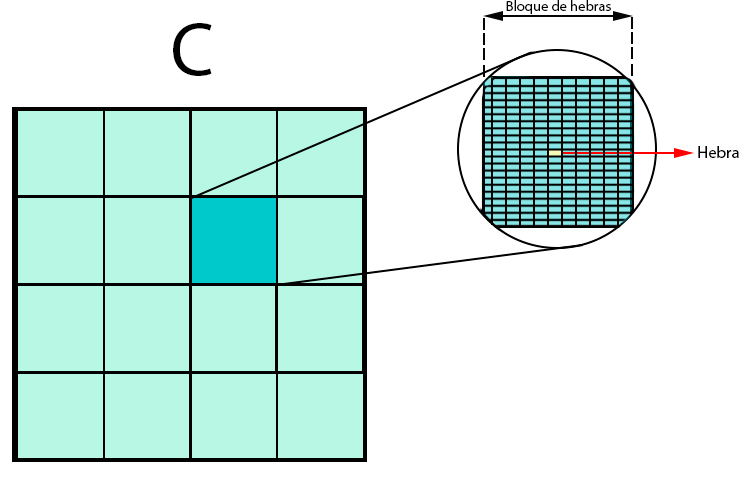
\includegraphics[scale=0.3]{imagenes/gemm_tile_v3.jpg}  
	\caption{Tercera implementación de multiplicación matricial con CUDA}
	\label{fig:mult_matrix_cuda_v3}
\end{figure}

Por tanto, resulta evidente la existencia de una ``tercera'' implementación carente de este gran defecto. Esta se caracteriza por la división la matriz C en submatrices o tiles, de forma que cada tile sea un bloque cuda. Partiendo de las implementaciones anteriores, el cambio resulta inmediato y los resultados descomunales pues aporta la capacidad de multiplicación matricial con independencia del tamaño de A y B, además de mejoras en cuanto a rendimiento. \cite{cuda_mult_matrix_v3} \\
Sin embargo, esta última implementación carece de los beneficios de la memoria compartida nivel de bloque, por lo que una vez más indica la muy posible existencia de una mejora sobre la misma. \\

\begin{figure}[H]
	\centering
	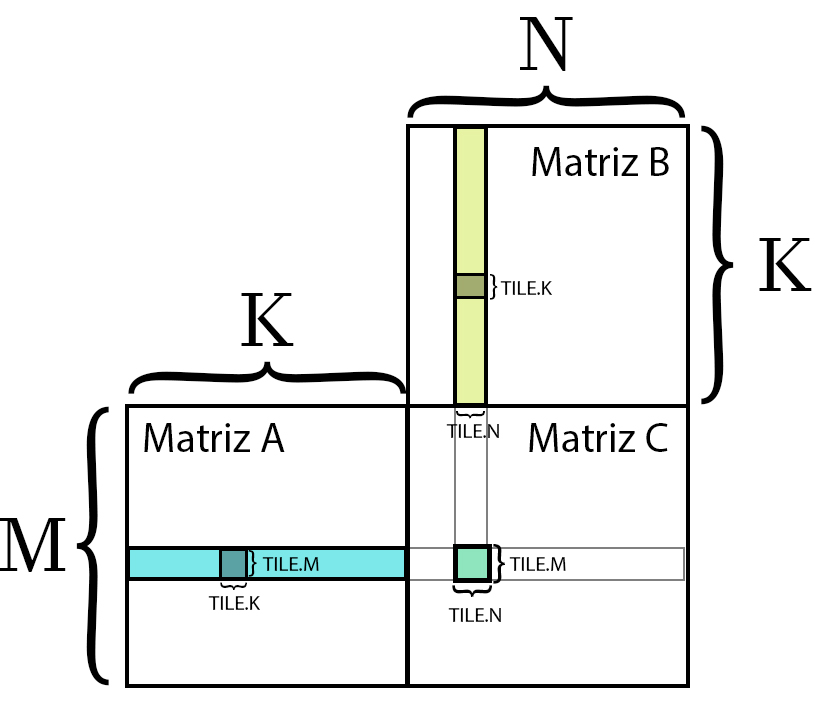
\includegraphics[scale=0.3]{imagenes/gemm_tile_v4.jpg}  
	\caption{Cuarta implementación de multiplicación matricial con CUDA}
	\label{fig:mult_matrix_cuda_v4}
\end{figure}
Para realizar el cálculo de cada valor de C es necesario multiplicar una fila de A por una columna de B. Es decir, multiplicar dos vectores de K elementos. Una idea inicial consiste en cargar 2K elementos en memoria compartida para posteriormente usarlos. Sin embargo, si cada hebra de cada bloque requiere 2K elementos, esto no es viable pues la memoria compartida es limitada y escasa. En su lugar, un mejor enfoque consiste en, dado un bloque 2D de dimensiones TILExTILE, almacenar 2*TILE*TILE. Su objetivo es dividir el cálculo de cada valor de C en iteraciones, y en cada una de ellas, cada hebra multiplica TILE elementos de A por TILE de B, además de acumular y sumar los resultados obtenidos en cada iteración. \cite{nvidia_mult_matrix_v4}
